%%%--------------------------------------------------------------------------------------------
\documentclass[a4paper, jou, natbib]{apa6}
\usepackage[english]{babel}
\usepackage[utf8x]{inputenc}
\usepackage{mathtools}
\usepackage{amssymb}
\usepackage{graphicx}
\usepackage[colorinlistoftodos]{todonotes} 
\usepackage{etoolbox}

\newtoggle{jou}
\toggletrue{jou}
%\togglefalse{jou}

%\usepackage{lineno}

\title{Temporal Distinctiveness in Task Switching: Assessing the Mixture-Distribution Assumption}
\shorttitle{Mixture Distribution Assumption}
\author{James A. Grange}
\affiliation{School of Psychology, Keele University, UK}

\note{{\bf Word Count:} x,xxx (Main body, not including abstract or references.)}
% \note{{\bf Under Review---Please, no direct quotes.}}

% command to insert editing comments or track changes
\newcommand{\jg}[1]{\textcolor{blue}{$^{\textrm{}}${#1}}}

%command for R symbol
   \newcommand{\R}{R}

\authornote{Please address correspondence to James A. Grange, School of Psychology, Dorothy Hodgkin Building, Keele University, Keele, UK, ST5 5BG. Email: grange.jim@gmail.com. All raw data, analysis code, and model code are available to download at http://bit.ly/1l22EUV.}

\leftheader{Grange}

\abstract{.}

\keywords{Task switching; decay; interference; computational model}

\begin{document}
\maketitle
%%%--------------------------------------------------------------------------------------------

%%%--------------------------------------------------------------------------------------------
\section{Behavioural Data}
Describe the gist of the method, and provide a plot of the pertinent data
%%%--------------------------------------------------------------------------------------------

%%%--------------------------------------------------------------------------------------------
\section{Assessing the Presence of Mixture-Distributions}
\cite{VanMaanen2014} introduced a method---the ``fixed-point'' property test---for statistically testing the presence of a mixture-distribution, given two ``base'' distributions. If distribution $z$ is a mixture of two base distributions $x$ and $y$, then the fixed-point property states that the probability density for distribution $z$, $f_{z}$, is a weighted sum of the probability densities of the other two distributions $f_{x}$ and $f_{y}$. Put simply, this implies that there exists a particular response time $t$ for which the probability of providing such as response is identical for all three distributions; that is $f_{x}(t)$ = $f_{z}(t)$ = $f_{y}(t)$. 

For example, consider the left panel of Figure \ref{fig:fpExample}. Here, three response time distributions have been simulated: $x$ is a fast RT distribution, and $y$ is a slow RT distribution. Distribution $z$ was simulated as being a mixture of distributions $x$ and $y$ with mixture probability $p$ set to $p$ = 0.7.  

\iftoggle{jou}{
\begin{figure}
\begin{center}
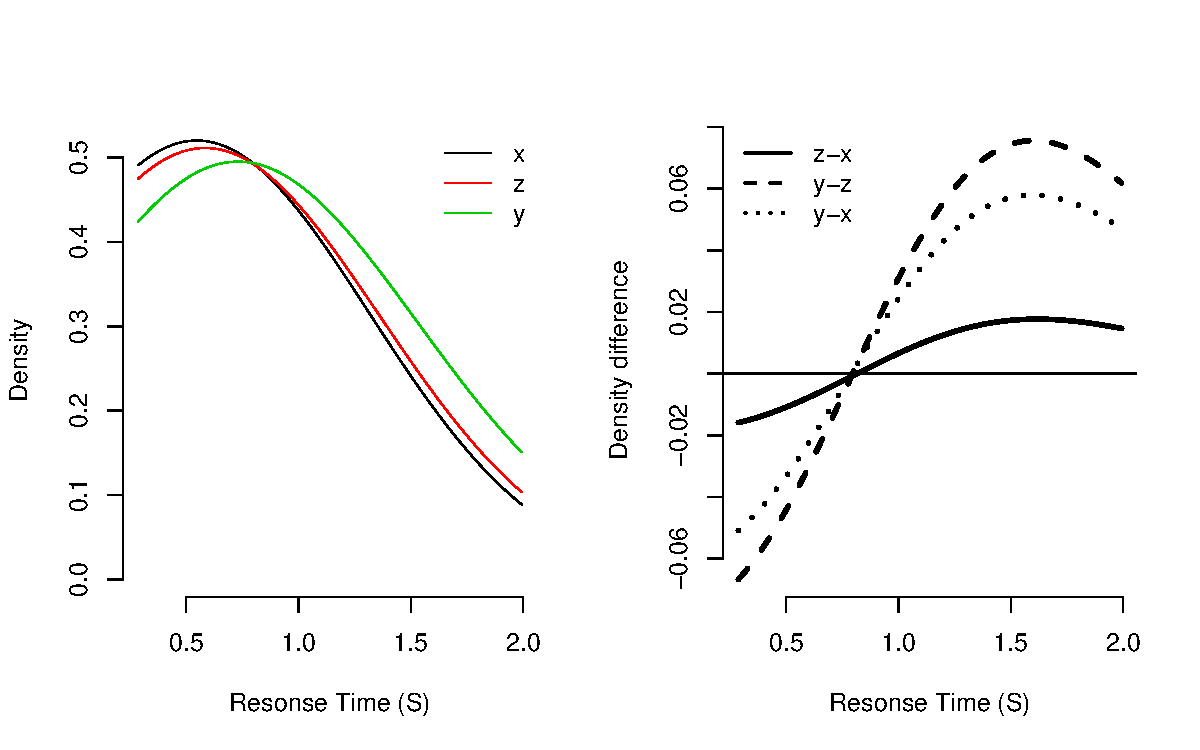
\includegraphics[width = 0.5\textwidth]{Images/fpExample.pdf}
\caption{Example of the fixed-point property in three distributions. Distribution $z$ is a mixture of distributions $x$ and $y$ with mixture probability $p$ set to $p$ = 0.7. The left panel shows the probability densities for each distribution. The right panel shows the density difference between different density functions. The distributions share a common crossing point at about 0.850 seconds.}
\label{fig:fpExample}
\end{center}
\end{figure}
}{
\begin{figure}
\begin{center}
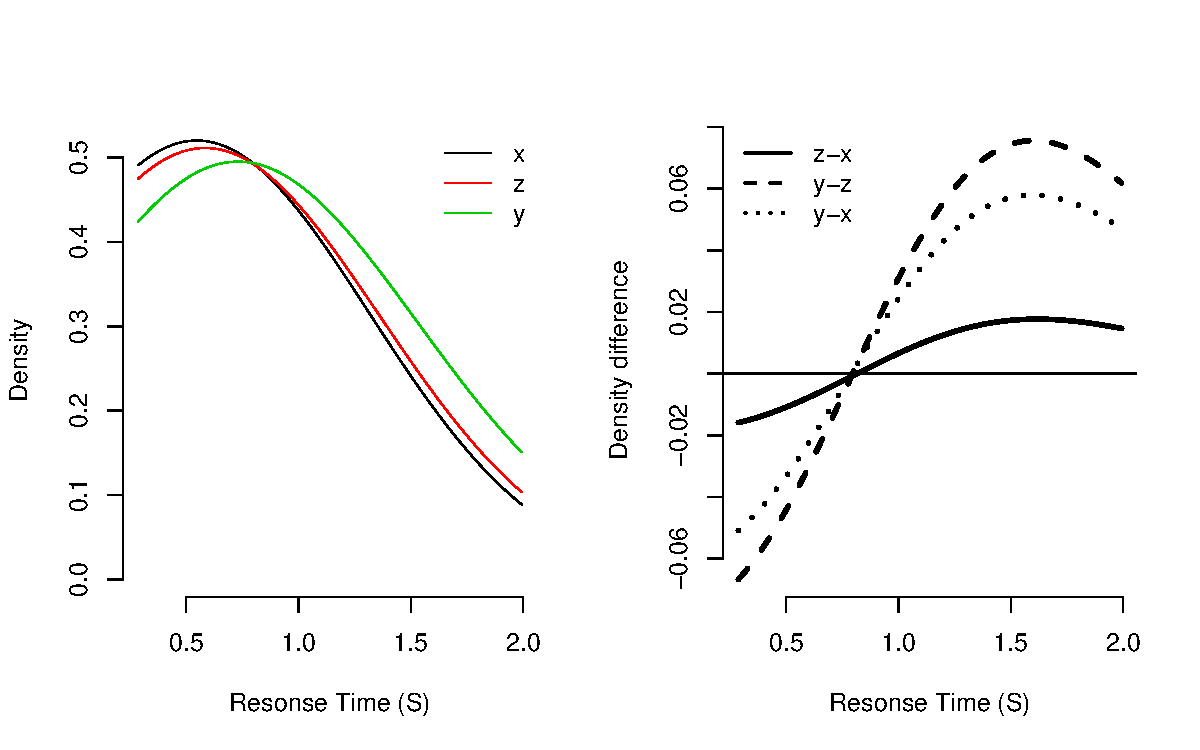
\includegraphics[width = \textwidth]{Images/fpExample.pdf}
\caption{Example of the fixed-point property in three distributions. Distribution $z$ is a mixture of distributions $x$ and $y$ with mixture probability $p$ set to $p$ = 0.7. The left panel shows the probability densities for each distribution. The right panel shows the density difference between different density functions. The distributions share a common crossing point at about 0.850 seconds.}
\label{fig:fpExample}
\end{center}
\end{figure}
}

As can be seen, the density functions of all three distributions share a common ``crossing point'', the RT at which all density functions are equal (i.e., where $f_{x}(t)$ = $f_{z}(t)$ = $f_{y}(t)$). The crossing point is made clearer by taking successive subtractions of pairs of density functions (see the right panel of Figure \ref{fig:fpExample}). Zero in this plot represents a density difference of zero (i.e., where the two density functions are equal). For example, the solid line represents the density difference of $f_{z}$ - $f_{x}$. If the distributions share a common crossing point, the density differences for all pairs of distribution differences will cross zero at a similar response time. This is the case in the current plot, where the three distributions share a common crossing point of about 0.850 seconds.

%%----------
\subsection{Application to the Data}
The data was assessed for the presence of a mixture distribution. Correct RTs were first trimmed to retain RTs slower than 150 milliseconds, and RTs faster than 2.5 standard deviations above each subjects' mean RT. The data was then assessed for the presence of a fixed-point by passing it to the \texttt{fp} function provided in the form of \texttt{R} code from \citet{VanMaanen2014}. Visual representation of the fixed-point assessment is shown in Figure \ref{fig:mixtureDistributionData}.

\begin{figure*}
\begin{center}
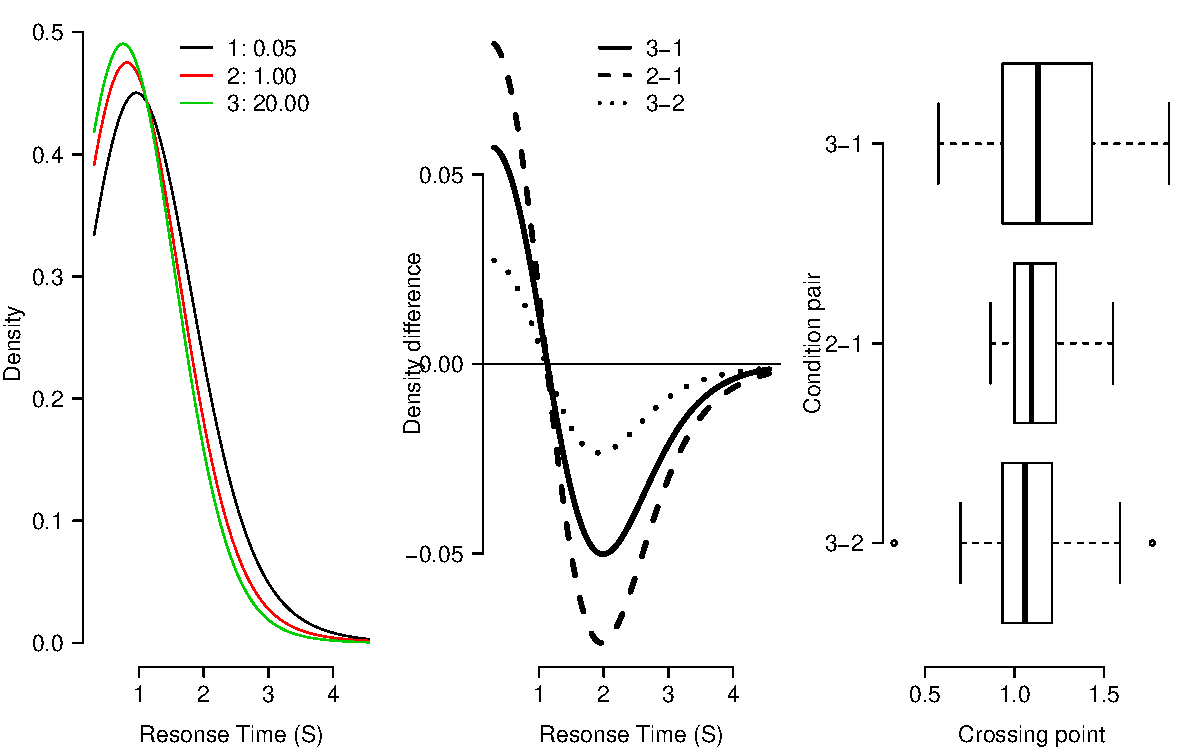
\includegraphics[width = \textwidth]{Images/mixtureDistributionData.pdf}
\caption{Example of the fixed-point property in three distributions. Distribution $z$ is a mixture of distributions $x$ and $y$ with mixture probability $p$ set to $p$ = 0.7. The left panel shows the probability densities for each distribution. The right panel shows the density difference between different density functions. The distributions share a common crossing point at about 0.850 seconds.}
\label{fig:mixtureDistributionData}
\end{center}
\end{figure*}

As shown in the left and center panels of Figure \ref{fig:mixtureDistributionData}, the three RT distribution functions share a common crossing point at just over 1 second. The right panel of Figure \ref{fig:mixtureDistributionData} shows boxplots of the distribution of crossing points for each pair for all subjects. There is considerable overlap in the boxplots suggesting no difference between condition pairs of crossing point (supporting the fixed-point hypothesis). Together, this visual inspection provides good evidence that the ratio = 1 RT function is a weighted mixture of the ``slow'' RT distribution (where ratio = 0.05) and the ``fast'' RT distribution (where ratio = 20), as predicted by the temporal distinctiveness model \cite{Grange2015}.

To assess statistical support for the common crossing point, a one-way ANOVA was conducted on the three levels of crossing-point pairs shown in the right panel of Figure \ref{fig:mixtureDistributionData}. The dependent variable in this analysis---shown in the x-axis of that Figure---is the crossing point in seconds for the density difference. This analysis was not statistically significant [\emph{F}(2, 48) = 1.25, \emph{p} = .295]. However, the presence of a common crossing point requires the acceptance of a null hypothesis (i.e., of no difference in crossing points), which cannot be achieved via standard statistical analysis. Therefore, a default Bayesian ANOVA \cite{Rouder2012} was conducted on the same data, which produces a Bayes Factor; the Bayes Factor---denoted $BF_{01}$---assesses the evidence in favour of a model assuming a common crossing point (i.e., a ``null'' model) compared to a model assuming multiple crossing points (i.e., an ``alternative'' model). The Bayes Factor for this data was $BF_{01}$ = 3.354, suggesting the data are 3.4 times more likely under the model assuming a common crossing point. Together, these statistical analyses converge on the conclusion that the RT distributions share a common crossing point, and as such can be considered support for the mixture-distribution hypothesis.

%%%--------------------------------------------------------------------------------------------
\section{A Mixture-Distribution Model of Temporal Distinctiveness Effects}

The previous section provided statistical support for the presence of a mixture-distribution for intermediate RCI ratios (i.e., intermediate levels of temporal distinctiveness). This is in agreement both with the verbal theory regarding TD effects \cite{Horoufchin2011a} and its formal implementation \cite{Grange2015}, which explains performance across TD ratios. In this section I develop a mathematical process model to predict RT distributions of TD data. The fitting of whole RT distributions presents an important advance over the model of \citet{Grange2015}, as it allows a direct test---rather than a relatively indirect test from fitting mean RTs---of that model's core assumption: that intermediate TD performance is a weighted mixture of ``retrieved'' and ``not-retrieved'' processing modes, which lead to fast and slow RTs, respectively. 

In this section, I first provide a schematic overview of the assumptions of the model. The mathematical details of the model are in Appendix B.

%%----------
\subsection{Overview of the Model}

\subsubsection{Episodic Retrieval}
The main processing stages in the model are shown in Figure \ref{fig:retrievalOverview}. The model assumes that, when presented with a task cue on a task repetition trial, the cognitive system attempts to retrieve the most recent episodic trace of this task (which was from trial n--1). The success of this retrieval attempt is influenced by the temporal distinctiveness of the episodic trace (at n--1) from a distracting episodic trace from the task two trials ago (at n--2).  

\iftoggle{jou}{
\begin{figure}
\begin{center}
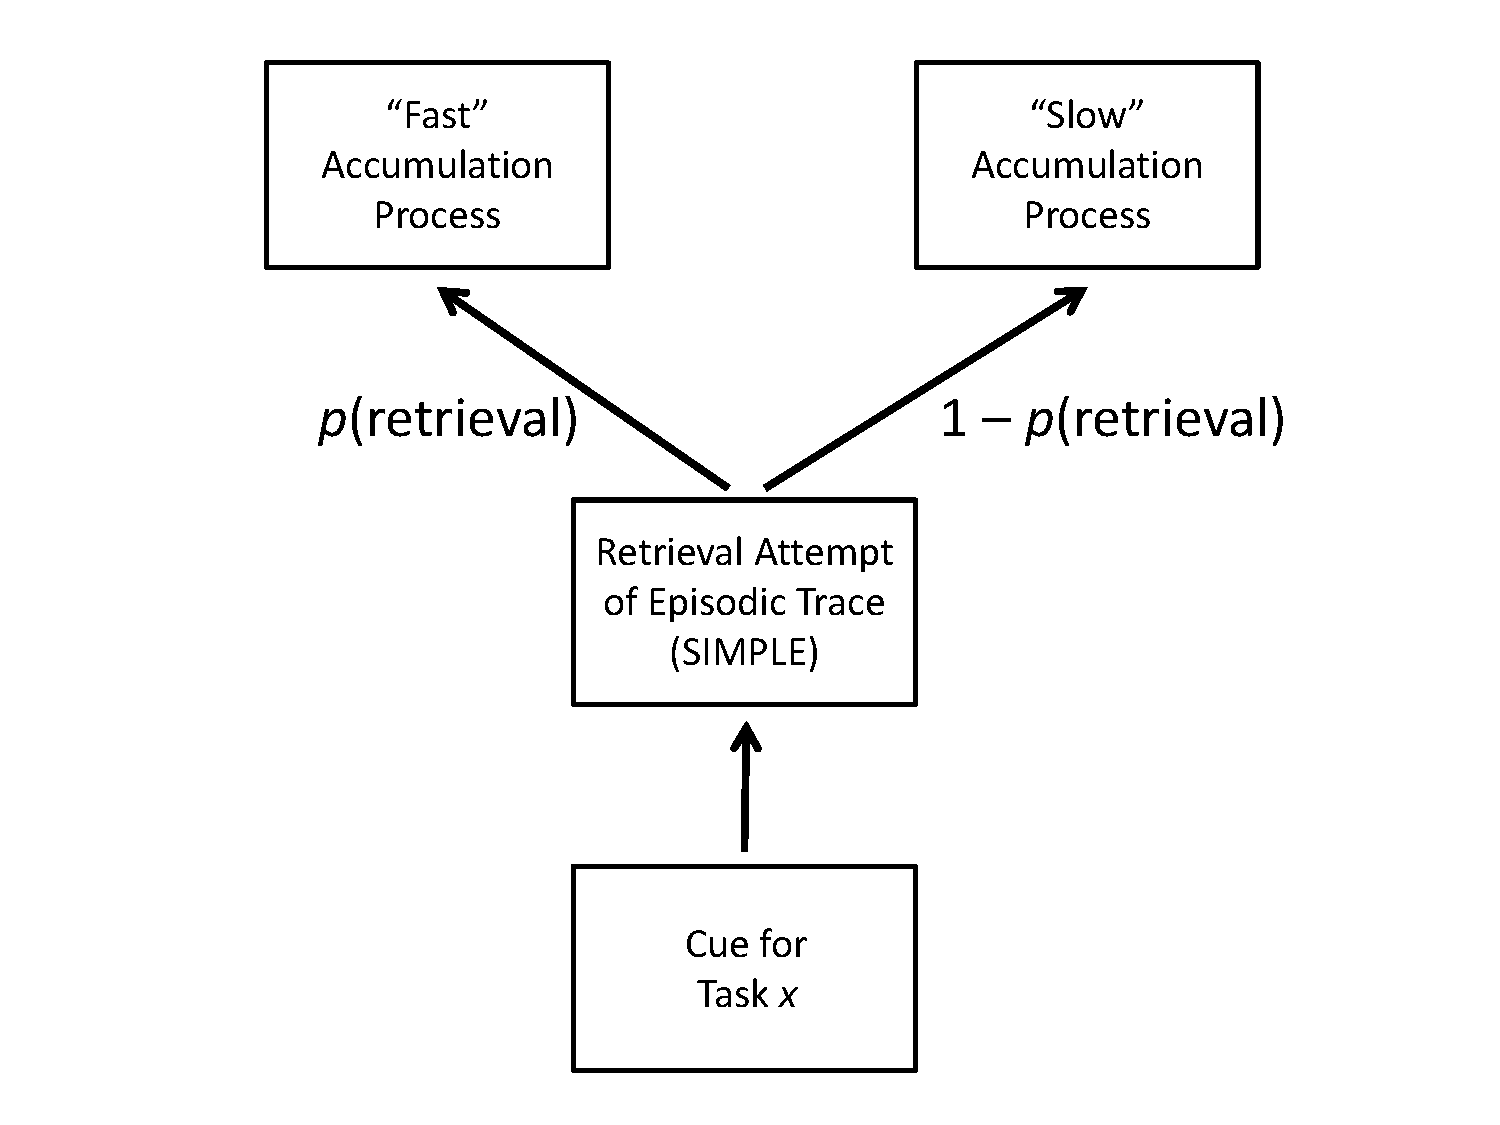
\includegraphics[width = 0.5 \textwidth]{Images/retrievalOverview.pdf}
\caption{Overview of the retrieval processes in the model.}
\label{fig:retrievalOverview}
\end{center}
\end{figure}
}{
\begin{figure}
\begin{center}
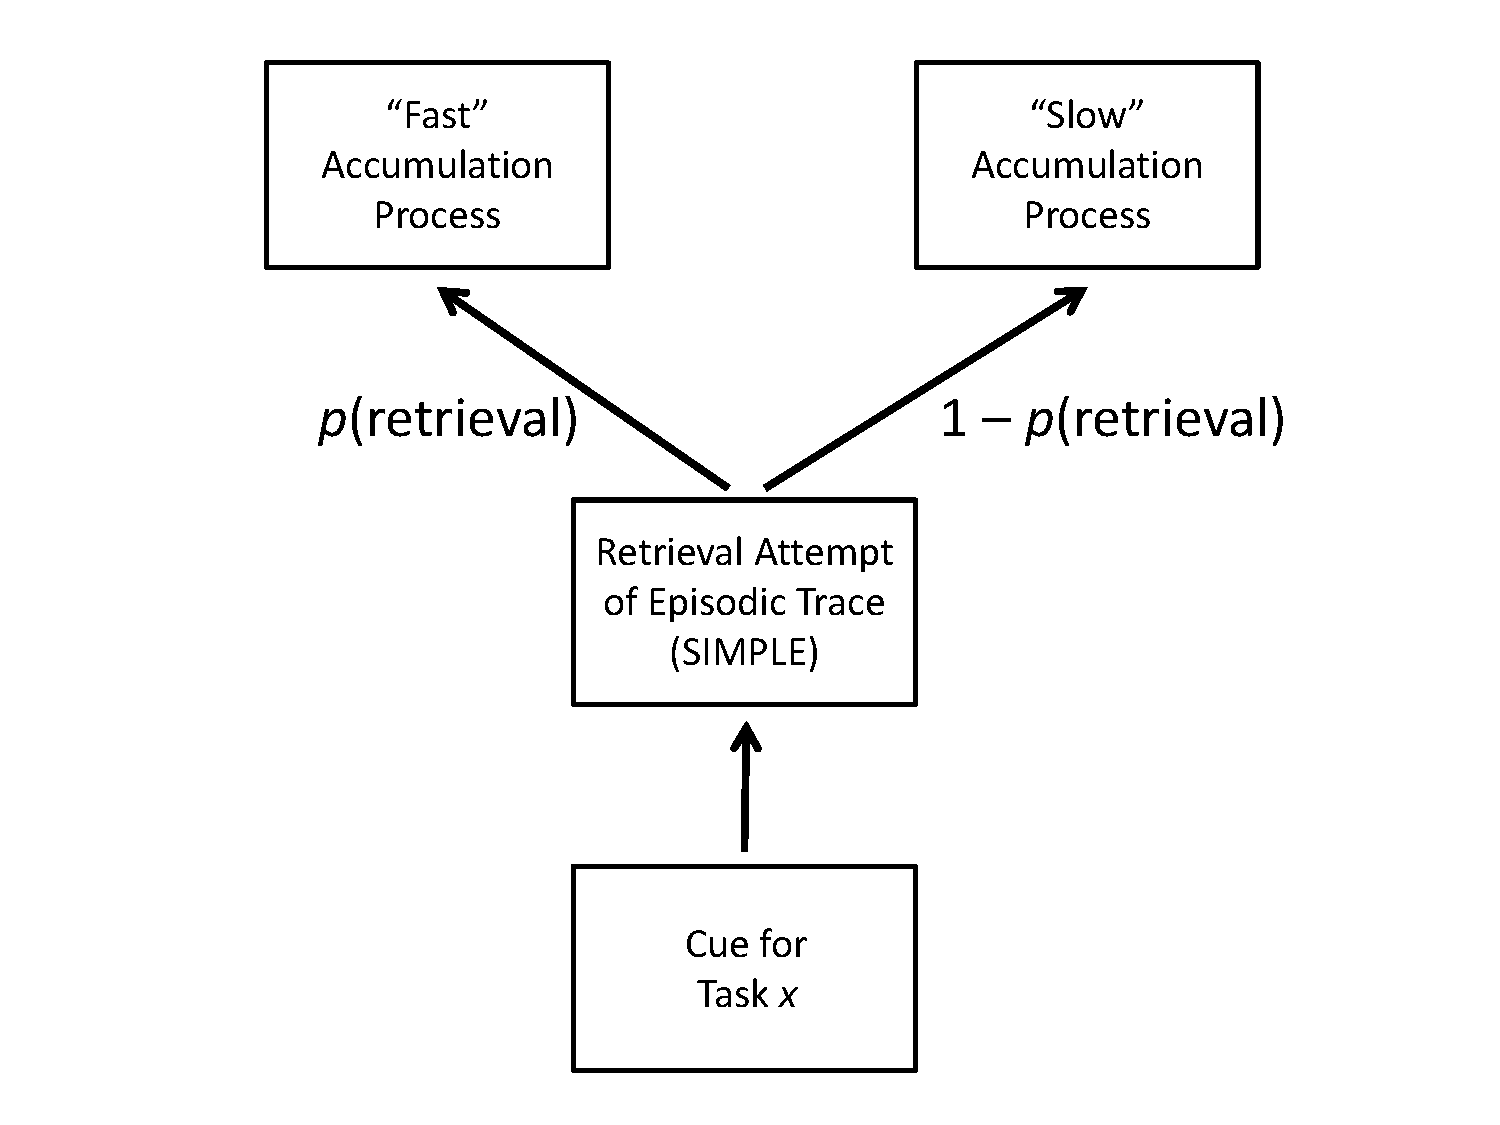
\includegraphics[width = \textwidth]{Images/retrievalOverview.pdf}
\caption{Overview of the retrieval processes in the model.}
\label{fig:retrievalOverview}
\end{center}
\end{figure}
}


Retrieval probability---$p$(retrieval)---influences the speed of retrieval. If retrieval succeeds, the response is facilitated due to retrieval of elements of the previous episodic trace that prime performance on the current trial; if retrieval fails, the response is not facilitated, and thus responding is slower as it has to be performed via a slower, algorithmic, route \citep[see][for discussion]{Grange2015}.

\subsection{RT Distributions}
To predict response time distributions, the mathematics of the Linear Ballistic Accumulator (ref) was used. The LBA is a successful model of choice response time, allowing the modelling of correct and error RT distributions. The model assumes that, when presented with a task stimulus, evidence accumulates towards a retrieval threshold. Evidence for each response---typically simplified to the ``correct'' and ``error'' response---accumulates in a linear fashion until one of the accumulators reaches the response threshold. At this point, it is assumed that this response has been selected by the model. 

The LBA model has several parameters. The mean rate of evidence accumulation is referred to as the \emph{drift rate}, $v$; it is larger for the correct response than for the error response. The drift rate for each accumulator can vary on each trial, but is assumed to have a fixed mean rate. The drift rate on each trial is a random draw from a normal distribution with mean $v$ and standard deviation $s$. The starting point of the accumulation process can vary uniformly between 0 and $A$. The height of the response threshold is governed by the parameter $b$. The time taken to perceptually encode stimuli and make a manual response is captured by a single non-decision time parameter $ter$. 

Figure \ref{fig:lbaAccumulation} shows how the LBA is applied in the current context. (Note that only the correct accumulators are shown to avoid clutter.) The model only ever uses one of two accumulation processes: If retrieval is successful, the model samples the current RT from a ``successful'', ``fast'' accumulation process with a higher drift rate, $v_{Fast}$; if retrieval fails, the current RT is sampled from an ``unsuccessful'', ``slow'' accumulation process with a lower drift rate, $v_{Slow}$. 

\iftoggle{jou}{
\begin{figure}
\begin{center}
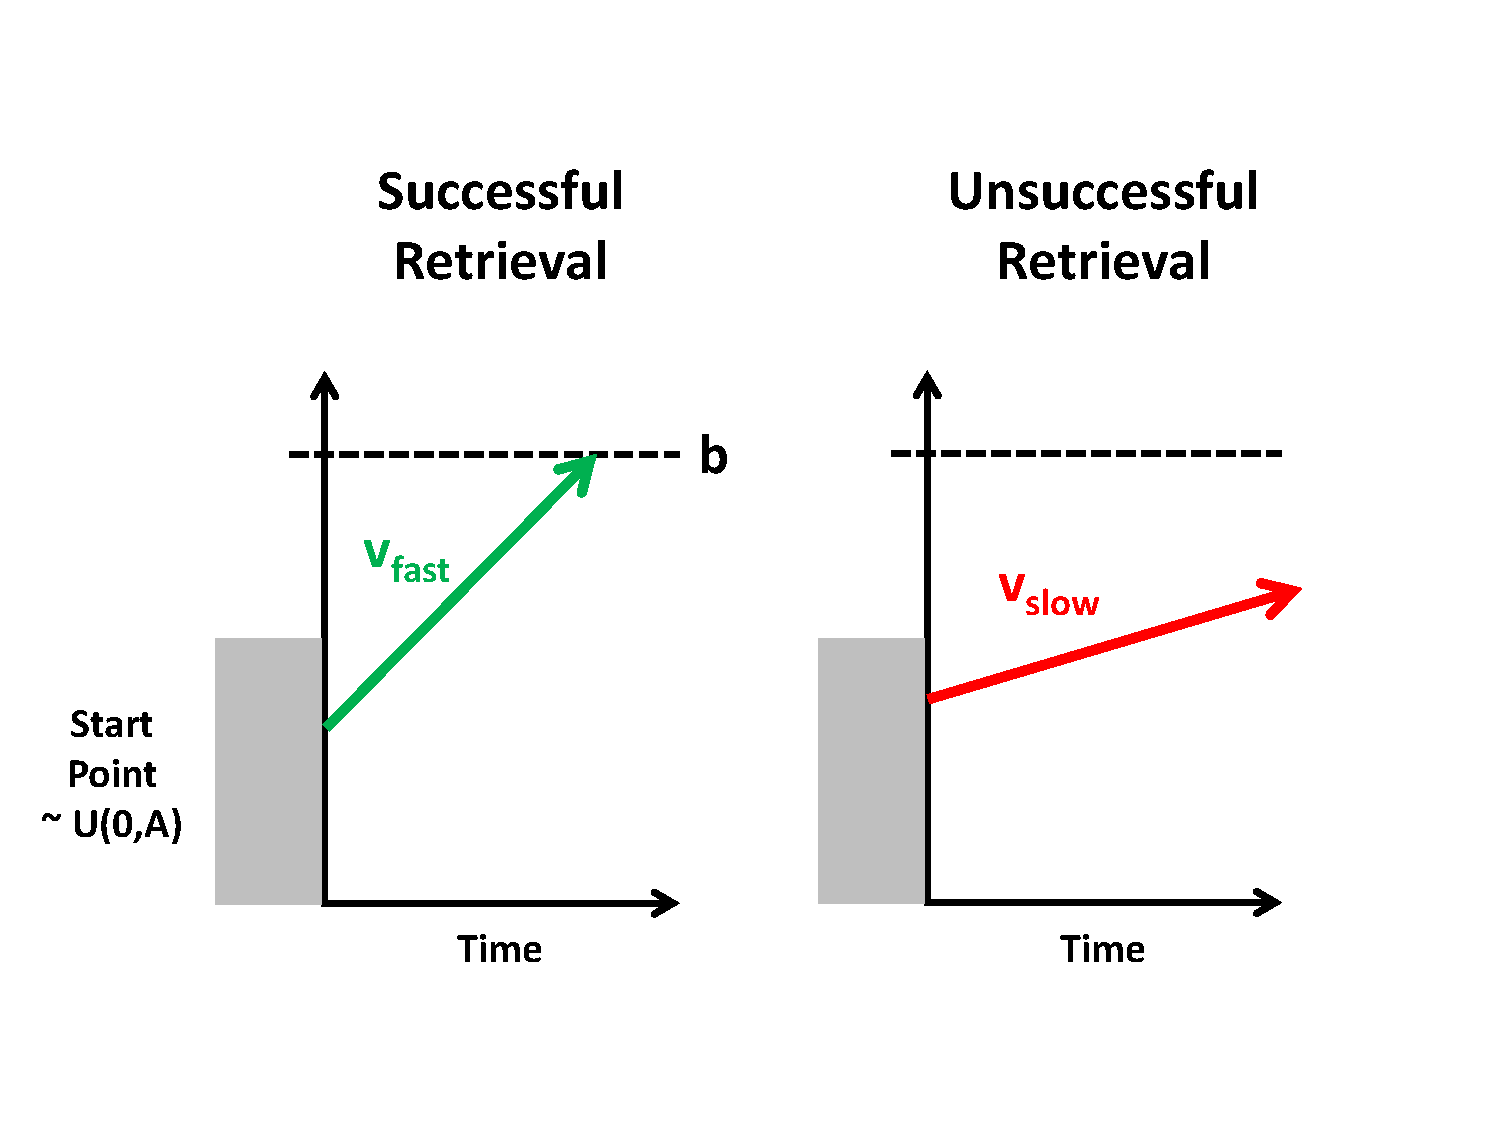
\includegraphics[width = 0.5 \textwidth]{Images/lbaAccumulation.pdf}
\caption{Overview of the Linear Ballistic Accumulation Process for successful and unsuccessful retrieval.}
\label{fig:lbaAccumulation}
\end{center}
\end{figure}
}{
\begin{figure}
\begin{center}
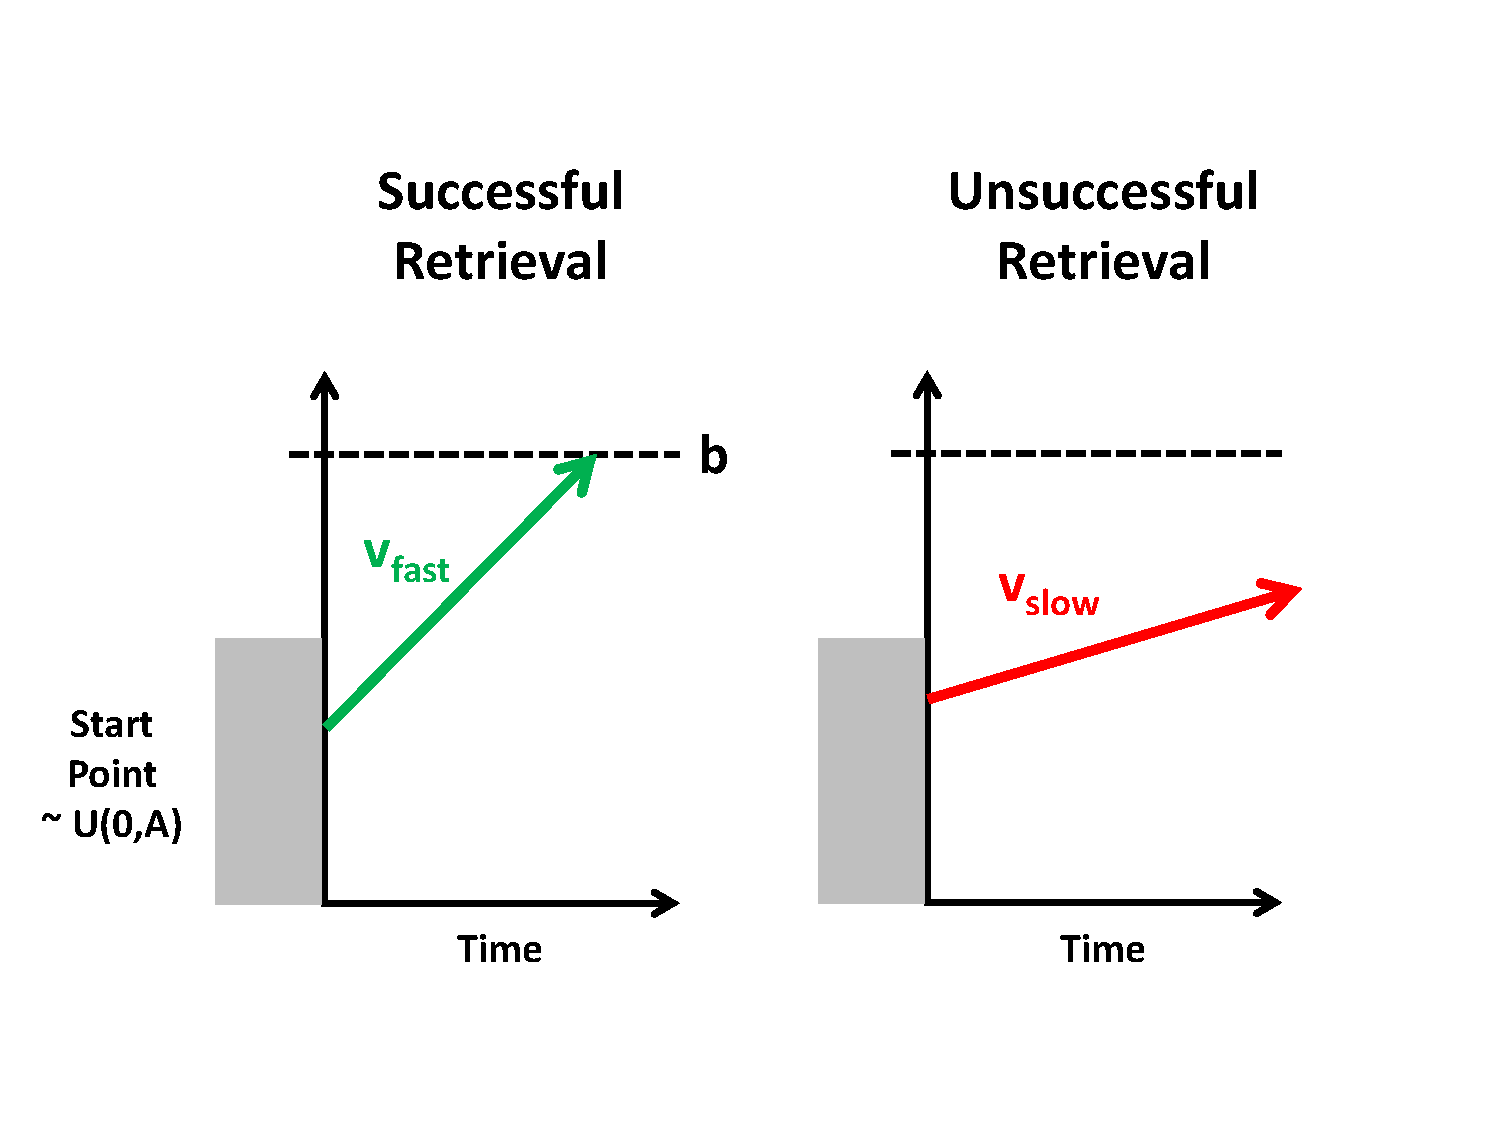
\includegraphics[width = 0.5 \textwidth]{Images/lbaAccumulation.pdf}
\caption{Overview of the Linear Ballistic Accumulation Process for successful and unsuccessful retrieval.}
\label{fig:lbaAccumulation}
\end{center}
\end{figure}
}


Thus, in this model, when TD is high, $p$(retrieval) is high, and as such more trials will be sampled from the fast accumulation process. When TD is low, so too will  $p$(retrieval), and as such more trials will be sampled from the slow accumulation process. Intermediate TDs will have an intermediate $p$(retrieval), and as such their RT distributions will be a weighed mixture of the two base distributions (fast and slow), with the exact proportion governed by $p$(retrieval). 

%%----------
\subsection{Fitting the Model}

\citet{Grange2015} used the full mathematics of SIMPLE to obtain $p$(retrieved). To reduce the number of free parameters, in the current model $p$(retrieved) was treated as a ``semi-fixed'' parameter. To acieve this, the TD ratio was calculated for each RCI-sequence condition in Figure (dataPlot). Specifically, the RCI ratio was 20 for n--2 to n--1 RCIs of 50ms--1000ms; the ratio was 1 for RCIs of 1000ms--1000ms and 50ms--50ms; and the ratio was 0.05 for RCIs of 50ms--1,000ms. 

$p$(retrieved) was ``semi-fixed'' in the sense that it was fixed at $p$(retrieved) = 1 for ratios of 20 (i.e., perfect retrieval) and fixed at $p$(retrieved) = 0 for ratios of 0.05 (i.e., failed retrieval); $p$(retrieved) was free to vary for ratios of 1. Thus, $p$(retrieved) controls the relative contribution of the two RT distributions for intermediate RCI ratios.

Separate drift rates were estimated for the ``fast'' and ``slow'' distributions---$v_{Fast}$ and $v_{Slow}$, respectively. (Note that drift rates for error response evidence accumulation is given as 1--$v$.) Also, each distribution had its own response threshold---$b_{Fast}$ and $b_{Slow}$.\footnote{Initial fits with just $v$ varying between the fast and slow distributions did not fit the data as well as when $b$ was also allowed to vary between conditions.} All other parameters (i.e., $A$, $s$, and $ter$ took on identical values for all three ratio conditions. 

Note therefore that this fit is rather ambitious. First, the model has to explain whole RT distributions for correct and error responses across all three conditions of RCI ratio; that is 30 data points with just 8 parameters. Also, the data for ratio = 1 is never explicitly modelled; rather, the model is fit to the ratio = 20 with a fast distribution and to ratio = 0.05 data with a slow distribution; the data for ratio = 1 is then estimated by a weighted contribution of the two distributions controlled only by $p$(retrieved)). 

The model was fitted to the data via a version of Quantile Maximum Probability Estimation (QMPE; REF), where the model is fit to RT quantiles rather than individual RTs as per maximum likelihood (see Appendix B for details). This method was used due to the relatively low number of trials per subject, and the rather low error rate. The fits of the model to the behavioural data are shown in Figure \ref{fig:modelFit}. 

% Table generated by Excel2LaTeX from sheet 'Sheet1'
\begin{table}[htbp]
  \centering
  \caption{Best fitting model parameters from the fit routine. Note that $p$(retrieved) refers to the probability of sampling from the fast distribution only for ratio = 1 data points. See text for details.}
    \begin{tabular}{rr}
    \toprule
    Model Parameter & Value \\
    \midrule
    $p(retrieved)$     & 0.759 \\
    $A$     & 718.14 \\
    $b_{Fast}$ & 114.58 \\
    $b_{Slow}$ & 179.96 \\
    $v_{Fast}$ & 1.132 \\
    $v_{Slow}$ & 0.893 \\
    $s$     & 0.44 \\
    $ter$   & 346.42 \\
    \bottomrule
    \end{tabular}%
  \label{tab:bestParameters}%
\end{table}%




\begin{figure*}
\begin{center}
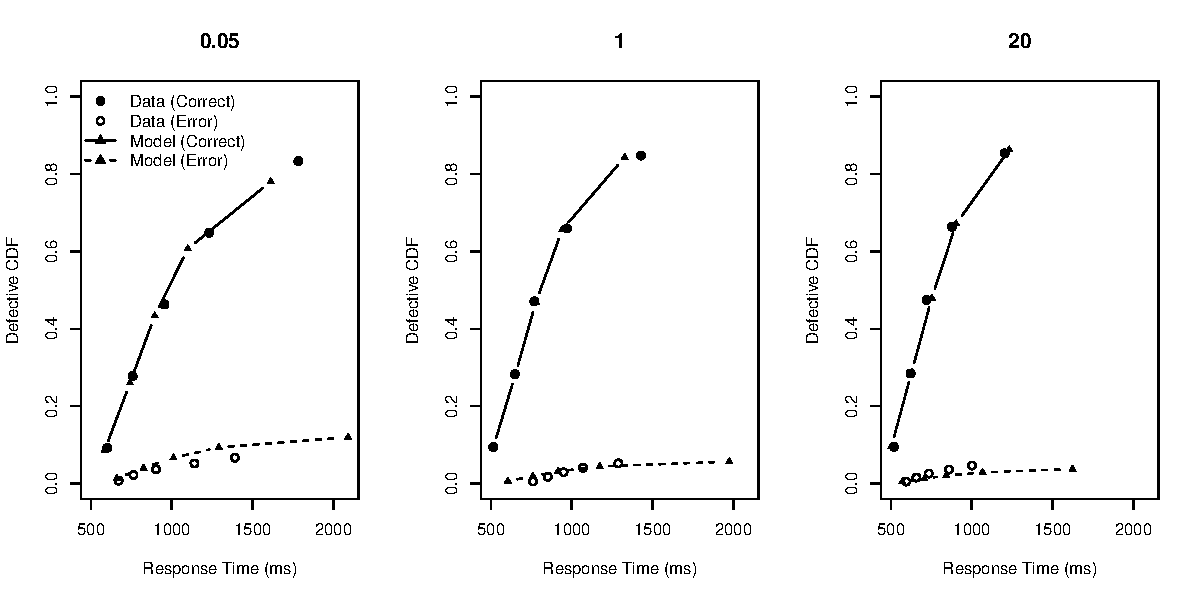
\includegraphics[width = \textwidth]{Images/qmp2RCI_drift_+_b.pdf}
\caption{Model fit.}
\label{fig:modelFit}
\end{center}
\end{figure*}

This Figure presents so-called ``defective'' cumulative distribution functions (CDFs). The data are sorted from fastest to slowest, and then quantile cut-off points are calculated for each subject according to a pre-specified set of quantiles $\vec{q}$ (here $\vec{q}$ = .1, .3, .5, .7, .9). The Figure plots the average RT for each quantile across subjects against the quantile value. The plot is a defective CDF in the sense that it also displays information about errors. Specifically, RT is plotted against $\vec{q}$ * mean accuracy rather than just $\vec{q}$. Error RT---shown in the Figure as open circles)---is error RT plotted against $\vec{q}$ * (1 - mean accuracy).

The model fit to correct RT distributions is rather good. The model captures all of the main trends in the data: RT becomes facilitated as $p$(retrieved) increases (from left-to-right $p$(retrieved) = 0, $p$(retrieved) = 0.759, and $p$(retrieved) = 1). This improvement in RT is largely at the slower end of the RT distribution. Also, the defective CDFs become steeper as $p$(retrieved) is increased, reflecting generally better accuracy. Importantly, the central plot shows a good fit of the model to the data, providing support that intermediate TDs are a mixture of two base distributions. 

The fit to the error RT distributions is not as good as for the correct RT distributions. However, accuracy was generally very high in this experiment (indeed, participants were excluded for not achieving greater than 90\% accuracy). So, there were often few error RTs per quantile bin during the model fit, making accurate estimation difficult. However, dispite the poor quantitative fit, the qualitative pattern seen in the human data is generally reproduced: error RT becomes generally faster and less variable as ratio increases.
%%%--------------------------------------------------------------------------------------------


%%%--------------------------------------------------------------------------------------------
\section{General Discussion}

%%%--------------------------------------------------------------------------------------------




%%%--------------------------------------------------------------------------------------------
\appendix
\section{Overview of Grange \& Cross (2015) Model}
The \citet{Grange2015} model used the mathematics of the SIMPLE \cite{Brown2007} model to account for TD effects on task repetition trials. Distinctiveness is proportional to the \emph{similarity} between a target trace and its neighbours in episodic memory. In this model, similarity is only influenced by the temporal domain. Similarity of instances at n--1 (item $i$) and n--2 (item $j$) is given by

\begin{equation}
\eta_{ij} = \left(\frac{T_{i}}{T_{j}}\right)^{c}, 
\label{eq:simpleSimilarity}
\end{equation}

\noindent where $T_{x}$ refers to the temporal age of an item. Temporal age is calculated from the current time. 

Based on the target traces $i$'s similarity, to its neighbours, its discriminability $D_{i}$ can be determined. This refers to how isolated the target trace $i$ is in episodic memory, and is given by

\begin{equation}
D_{i} = \frac{1}{\sum\limits_{j = 1}^n \eta_{ij}}.
\label{eq:simpleDiscriminationA}
\end{equation}

As we are only considering the similarity between two items ($i$ and $j$), and as an item's similarity to iself is 1, Equation \ref{eq:simpleDiscriminationA} becomes

\begin{equation}
D_{i} = \frac{1}{\sum\limits_{j = 1}^n \eta_{ij} + 1}.
\label{eq:simpleDiscriminationB}
\end{equation}

Given an item's discriminability, we can calculate its retrieval probability $p(R_{i})$ at time of retrieval $t$ by

\begin{equation}
p(R_{i}|D_{i}) = \frac{1}{1 + e^{-s(D_{i} - t)}}, 
\label{eq:simpleProb}
\end{equation}

\noindent where $s$ and $t$ are free parameters which descibe the sloe of the transforming function and the threshold of retrieval, respectively. 

Given these equations, we can calculate the retrieval probability for each level of temporal distinctiveness in the behavioural experiment. It is assumed that if the trace is retrieved (with probability $p$) then response time will be a random draw from a fast RT distribution with mean $\mu_{fast}$; if retrieval fails (with probability $1 - p$), the response time will be a random draw from a slow RT distribution with mean $\mu_{slow}$. Thus, mean RT for each level of TD is given by the RT-mixture equation

\begin{equation}
RT = p\mu_{Fast} + (1 - p)\mu_{slow}.
\label{eq:tdMixtureNew}
\end{equation}
%%%--------------------------------------------------------------------------------------------
\appendix
\section{Mixture-Distribution Model Details}

\subsubsection{LBA for Unitary Process}
In the LBA for a unitary process (i.e., not a mixture model), evidence for response $i$ has a CDF (at time \emph{t}) of

\begin{equation}
\begin{aligned}
F_{i}(t) = & 1 + \frac{b - A - tv_{i}}{A} \Phi\left(\frac{b - A - tv_{i}}{ts}\right) - 
\frac{b - tv_{i}}{A} \Phi\left(\frac{b - tv_{i}}{ts}\right) + \\ 
&\qquad \frac{ts}{A} \phi \left(\frac{b - A - tv_{i}}{ts}\right) - \frac{ts}{A} \phi \left(\frac{b - tv_{i}}{ts}\right),
\end{aligned}
\label{eq:lbaCDF}
\end{equation}

\noindent (where $\Phi$ refers to the normal distribution's CDF) and a PDF of 

\begin{equation}
\begin{aligned}
f_{i}(t) = \frac{1}{A} & \Biggl[-v_{i}\Phi \Biggl(\frac{b - A - tv_{i}}{ts}\Biggr) + s\phi\Biggl(\frac{b - A - tv_{i}}{ts}\Biggr) \\
&\qquad + v_{i}\Phi \Biggl(\frac{b - tv_{i}}{ts}\Biggr) - s\phi\Biggl(\frac{b - tv_{i}}{ts}\Biggr)\Biggr] 
\end{aligned}
\label{eq:lbaPDF}
\end{equation}

\noindent where $\phi$ refers to the normal distribution's density. Considering two accumulators $i$ and $j$ (e.g., correct \& error response, respectively), the PDF for $i$ at time $t$ is given by

\begin{equation}
\mbox{PDF}_{i}(t) = f_{i}(t) \prod_{j \neq i} \left(1 - F_{j}(t)\right).
\label{eq:defectivePDF}
\end{equation}


\subsubsection{Modelling Mixture Distributions}
If we denote the fast accumulation process as $\gamma$ and the slow accumulation process as $\lambda$, recall that mean RT can be predicted by

\begin{equation}
RT = p\mu_{\gamma} + (1 - p)\mu_{\lambda}.
\end{equation}

Extending this mixture model to a likelihood function, we can now obtain the PDF for response $i$ (rather than response $j$) at time $t$ by 

\begin{equation}
\begin{aligned}
\mbox{PDF}_{i} = &\left[p \cdot f_{\gamma i}(1 - F_{\gamma j})\right] + \\ 
&\qquad \left[(1 - p) \cdot f_{\lambda i}\right] (1 - F_{\lambda j})
\end{aligned}
\label{eq:tdLikelihood}
\end{equation}


\bibliography{References.bib}

\end{document}
